\chapter{Multi-Sweep-Line Algorithm}
\label{chap:methodology}
In this chapter, we formally present the problem and describe our parallel implementations. 

%Version 1 uses line sweep algorithm straightforward. Version 2 makes modifications based on version 1. In our implementation, we calculate the union area of rectangles on GPU and the triangles on CPU.

\section{Problem definition}
The input is a layout of VLSI design, which is a two dimensional rectangle space called a cell.  A cell is further subdivided into equal sized windows, whose width and height are equal to window size.  The window stride means the distance between two adjacent windows.  Inside the layout, components are decomposed as rectangles and triangles. The problem is to calculate the layout density of each window, which is the ratio of the area covered by rectangles and triangles. We only consider the union of rectangles here, and will discuss the process of union of triangles later.  Figure \ref{fig:fig_3_1} gives an example, in which the size and the stride of windows are the same.

\begin{figure}[!h]
    \centering
    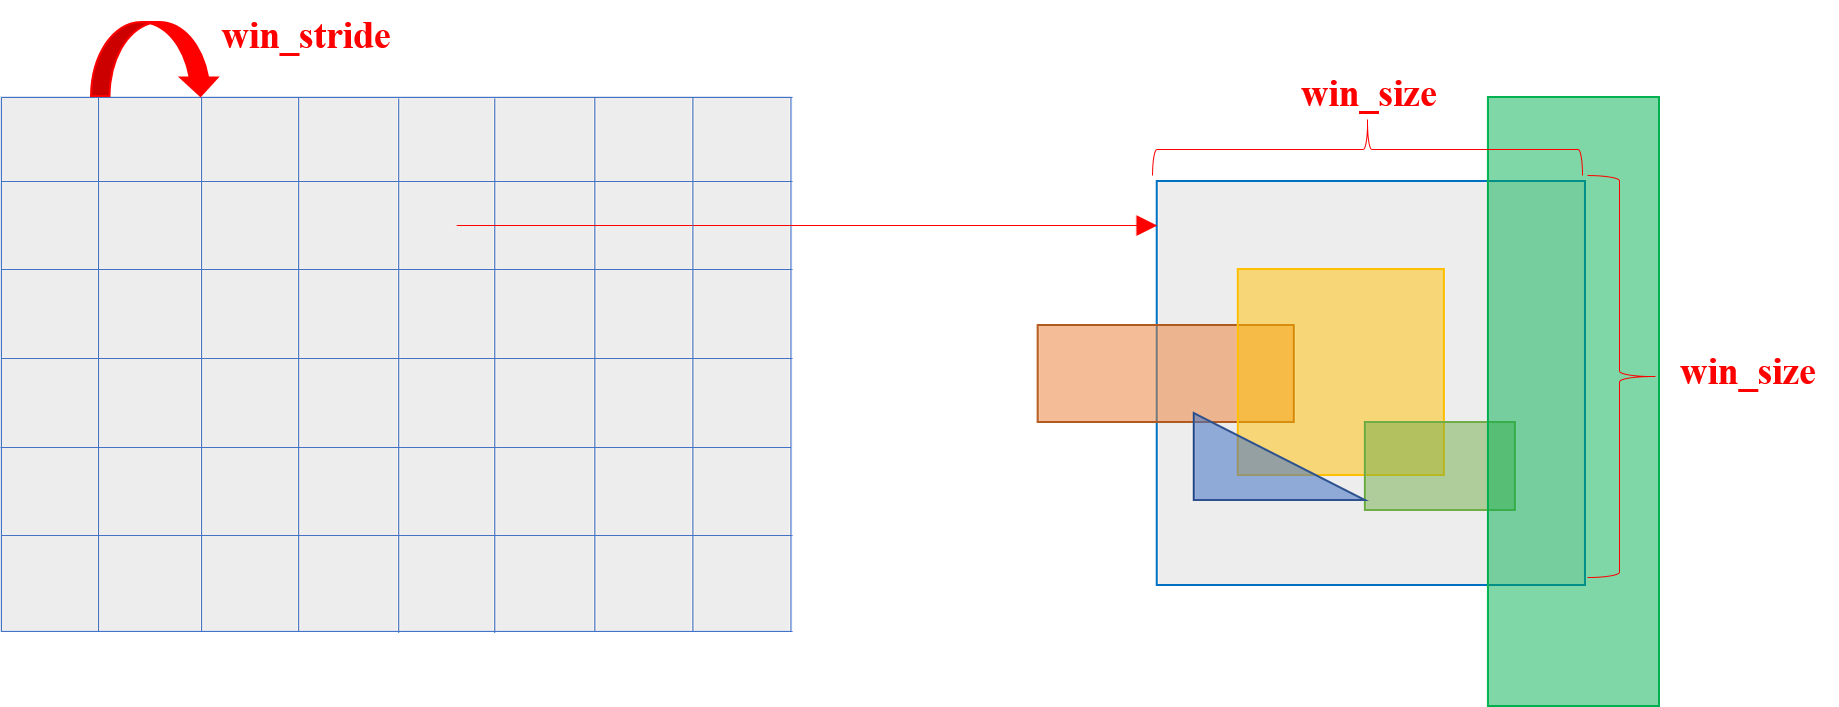
\includegraphics[scale=0.4]{image/fig_3_1}
    \caption{Cell, windows (window's stride is equal to size in this diagram), rectangles, and triangles}
    \label{fig:fig_3_1}
\end{figure}

\section{High Level Description}
% how to parallelize v1 v2 v3
In this section, we describe our three parallel implementations: baseline, multi-slab, and multi-sweep-line in high level.

\subsection{Baseline Algorithm}
Our baseline version is embarrassing parallelization. A layout can be partitioned into windows, so we can compute the union of rectangles for each window in parallel. In baseline version, we use sweep line algorithm and directly port it to GPU. The pseudo code is shown in Algorithm \ref{alg:a2}. To reduce the memory usage, we do not save y value. 

\begin{algorithm}[H]
\label{alg:a2}
\caption{Baseline: sweep line algorithm directly porter}
\DontPrintSemicolon
\renewcommand\baselinestretch{0.7}\selectfont
 \KwData{$R$: a list of rectangles for each window}
 \KwResult{Each window's area of rectangle union}
 \SetKwProg{Fn}{Function}{}{}
 \SetKwFunction{FMain}{main}
 \SetKwProg{Pn}{Function}{:}{\KwRet}
 \Pn{\FMain}{
     sort the x value of rectangles for each window\;
     sort each window's rectangles based on y\;
     \bf{parallel} \ForEach{$W_j \in W$}{
         $area = 0$\;
         \bf{parallel} \ForEach{$slab (x[i-1], x[i])$}{
             compute\_area($x[i-1], x[i]$)\;
         }
     }
 }
 \;
 \Pn{compute\_area($x1, x2$)}{
    Let $R[k]$ be the first rectangle in $[x1, x2]$\;
    begin = R[k].ymin\;
    end = R[k].ymax\;
    \ForEach{$r \in R$}{
        \If{$r$ is in $[x1, x2]$}{
            \uIf{$r.ymin <= end$}{
                $end = max(r.ymax, end)$\;
            }
            \Else{
                $area += (end - begin) * (x2 - x1)$\;
                $begin = r.ymin$\;
                $end = r.ymax$\;
            }
        }
    }
 }
\end{algorithm}

\subsection{Multi-Slab Algorithm}
The function of computing\_area in baseline version (naive parallelization) is the performance bottleneck because each thread checks all rectangles in a window, whether a rectangle is in the slab or not. It is ineffective for GPU architecture. For this reason, we modified the implement by changing threads' task. Each thread now handles one slab and only checks the rectangles in this slab. The pseudo code of compute\_area function is shown in Algorithm \ref{alg:a3}.

\begin{algorithm}[H]
\label{alg:a3}
\caption{Multi-slab: modify bottleneck in baseline and task partition}
\DontPrintSemicolon
\renewcommand\baselinestretch{0.7}\selectfont
 \KwData{$R$: a list of rectangles for each window}
 \KwResult{Each window's area of rectangle union}
 \SetKwProg{Fn}{Function}{}{}
 \SetKwFunction{FMain}{main}
 \SetKwProg{Pn}{Function}{:}{\KwRet}
 \Pn{\FMain}{
     sort the x value of rectangles for each window\;
     sort each window's rectangles based on y\;
     create active list for each slab each window\;
     \bf{parallel} \ForEach{$W_j \in W$}{
         $area = 0$\;
         \bf{parallel} \ForEach{$slab (x[i-1], x[i])$}{
             compute\_area($x[i-1], x[i]$)\;
         }
     }
 }
 \;
 \Pn{compute\_area($x1, x2$)}{
    Let $r1$ be the first rectangle in $[x1, x2]$\;
    begin = r1.ymin\;
    end = r1.ymax\;
    \ForEach{$r \in R$}{
        \uIf{$r.ymin <= end$}{
            $end = max(r.ymax, end)$\;
        }
        \Else{
            $area += (end - begin) * (x2 - x1)$\;
            $begin = r.ymin$\;
            $end = r.ymax$\;
        }
    }
 }
\end{algorithm}

\subsection{Multi-Sweep-Line Algorithm}
In the function of compute\_area in multi-slab version, each thread handles a slab and scan all rectangles within this slab. It is faster than the compute\_area function in baseline version. However, it suffers from the discontinuous memory access. So we present multi-sweep-line algorithm to speed up the computing time in compute\_area function. The pseudo code of compute\_area function is shown in Algorithm \ref{alg:a4}.

\begin{algorithm}[H]
\label{alg:a4}
\caption{The compute\_area function in multi-sweep-line which is optimized from multi-slab version}
\DontPrintSemicolon
\renewcommand\baselinestretch{0.7}\selectfont
\SetKwProg{Pn}{Function}{:}{\KwRet}
 \Pn{compute\_area($x1, x2$)}{
    //multi sweep line\;
    warp (32 thread) task:\;
    each warp handles a slab\;
    \While{choose 32 rectangles}{
        each thread handles a rectangle\;
        check rectangles before this thread\;
        add result to area\;
    }
 }
\end{algorithm}

%%%%%%%%%%%%%%%%%%%%%%%%%%%%%%%%%%%%%%%%%%%%%%%%%%5
\section{GPU Implementation}
In this section, we describe our three parallel implementations: baseline, multi-slab, and multi-sweep-line more detailed.

\subsection{Baseline Algorithm}
The layout density calculation can be parallelized embarrassingly by computing the density of each window in parallel, and then aggregating all the results.  We designed an effective GPU implementation for this method so that we can use it as the baseline for comparison.  The implementation uses four global arrays:
\begin{itemize}
    \item Counter Array ($C$): whose size equals to the number of windows.  Element $C[i]$ records the number of rectangles in window $i+1$.
    \item Offset Array ($O$): whose size also equals to the number of windows.  Elements in $O$ represent the indices of Rectangle Array ($R$).  
    \item Rectangle Array ($R$): whose size equals to the total number of rectangles in all windows, $\sum_{i=1}^n C[i]$.  The IDs of rectangles in window $i$ are stored in $R$ from index $O[i-1]$ to index $O[i]-1$, or to the last element of $R$.
    \item X\_range Array ($X$): whose size is double of that of $R$. It stores the x coordinates of two end points of rectangles in each window.
\end{itemize}
Fig. \ref{fig:fig_3_3} shows an example of those data structures.  
\begin{figure}[h]
    \centering
    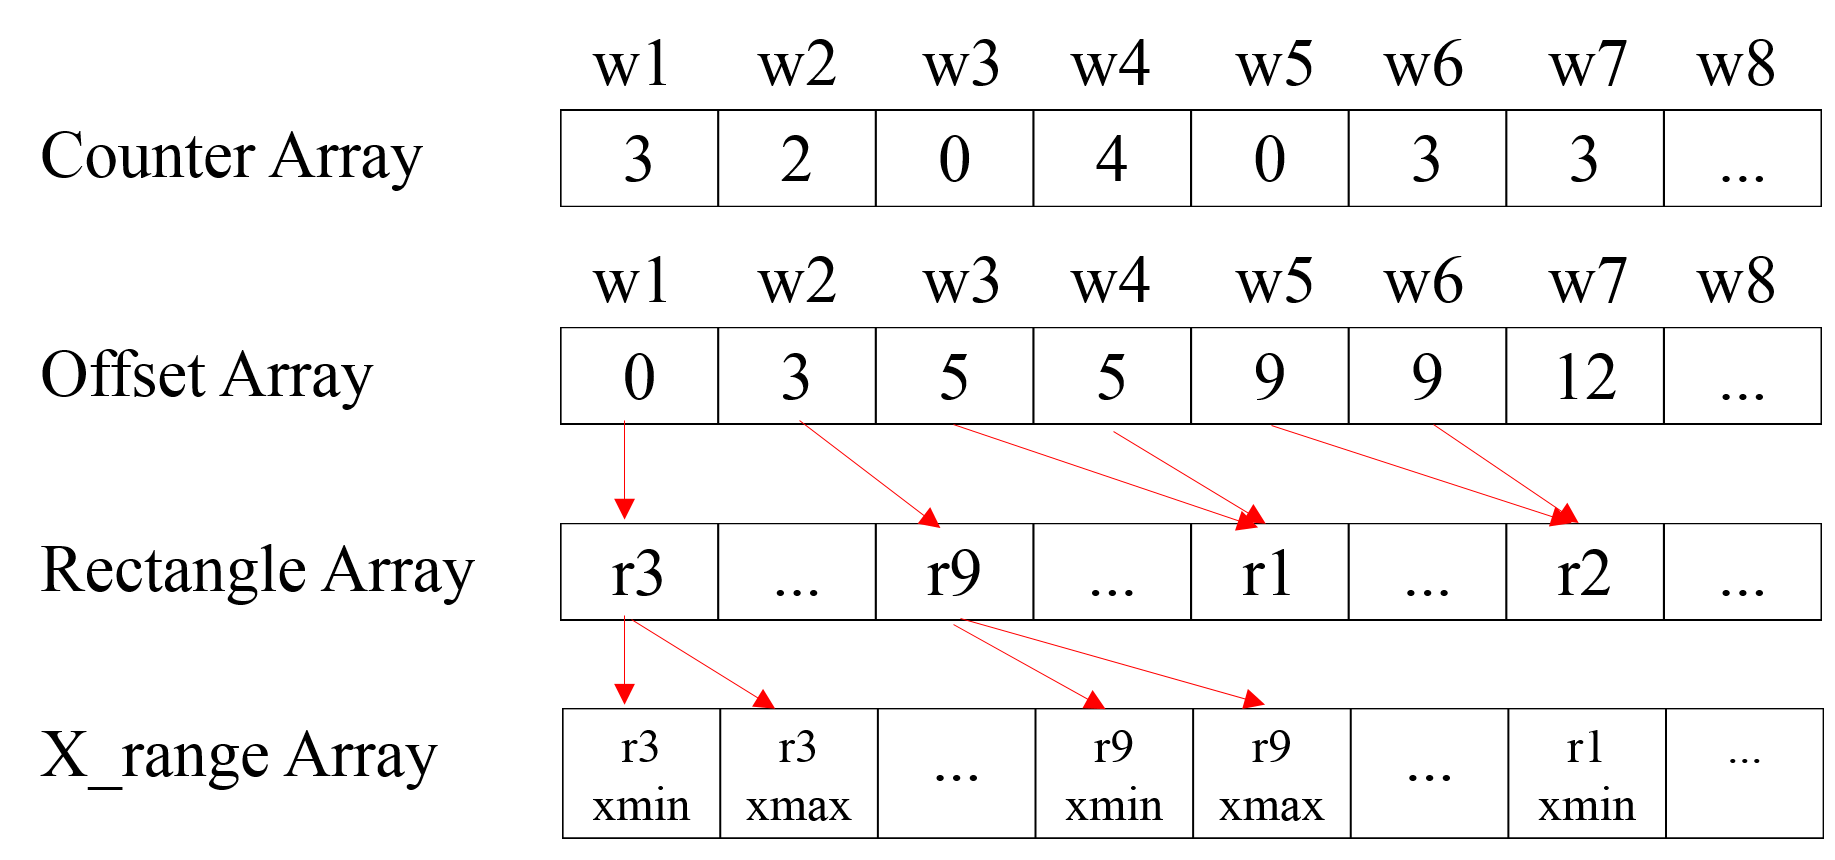
\includegraphics[scale=0.4]{image/fig_3_3}
    \caption{Example of the counter, offset, rectangle, and x\_range array. Rectangles are concatenated in the rectangle array according to the cell order}
    \label{fig:fig_3_3}
\end{figure}


The algorithm consists of three phases: counting phase, mapping phase, and computing phase.  The first two phases enumerate the rectangles appeared in each window and store their information using those four arrays.  The rectangles are sorted first based on their y coordinates, so the algorithm can process the rectangles sequentially later.  The last step calculates the area union of rectangles.

The counting phase counts the number of rectangles in each window.  Each thread handles a rectangle and computes which windows it occupies.  If a rectangle appears in window $i$, the thread increases the $i$th element of the \textit{counter array} $C$ using atomic instructions.

The target of mapping phase is to fill the \textit{rectangle array} with rectangles' ID. First, it uses the \textit{counter array} and performs parallel prefix sum algorithm (scan) \cite{ref} to generate the \textit{offset array}. Second, it fills the \textit{rectangle array} with rectangles' ID. The position of a rectangle in the \textit{rectangle array} is the \textit{offset array} of the window.  Each thread handles a rectangle and performs one atomic add instruction to obtain the correct order in the \textit{rectangle array}.  When filling the rectangle to the \textit{rectangle array}, it also fills the \textit{x\_range array}.  Finally, the algorithm sorts every segment of the \textit{rectangle array} and the \textit{x\_range array} to ensure the order of rectangles and slabs. 

The computing phase uses sweep line algorithm to calculate the density of rectangles in each window. Each block processes four windows.  Each thread picks one slab to compute the union area and repeats the action until all slab are computed. Every thread reads the information of all the rectangles in the window. If the rectangle is not appeared on the range (slab), the thread will ignore it. When sweeping rectangles in the window, each thread performs one atomic instruction to shared memory to record the area covered by rectangles. Finally, the algorithm writes the answer from the shared memory to the global memory.
\begin{figure}[h]
    \centering
    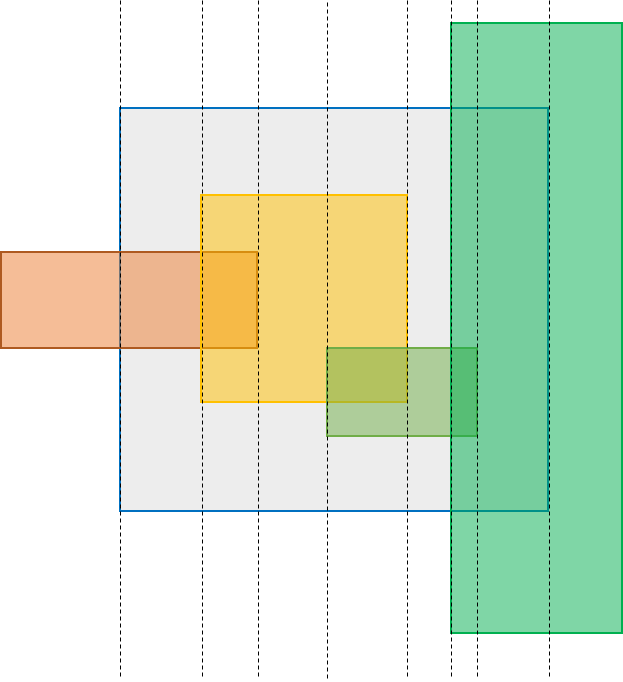
\includegraphics[scale=0.4]{image/fig_3_4}
    \caption{Computing phase: each thread handles a slab (between two dash line)}
    \label{fig:fig_3_4}
\end{figure}


The bottleneck of the baseline algorithm is in the computing phase because each thread needs to check all rectangles in a window, whether they are in the slab or not.  

\subsection{Multi-Slab Algorithm}
The computing phase in baseline version (naive parallelization) is the performance bottleneck because each thread checks all rectangles in a window, whether a rectangle is in the slab or not. It is ineffective for GPU architecture. For this reason, we modified the implement by changing threads' task. Each thread now handles one slab and only checks the rectangles in this slab.

Our target is to generate an array to store the concatenated rectangles lists for all slabs for all windows. For this purpose, three additional arrays are used. First, the \textit{range rectangle array} stores the concatenated rectangles lists for all slabs for all windows. Second, the \textit{range offset array} records the beginning address of each rectangle list in the \textit{range rectangle array}. Third, the \textit{range counter array} keeps the number of rectangles in each slab for all windows. Fig. \ref{fig:fig_3_5}a shows the flow chart of multi-slab version. Multi-slab version consists of five phases, which are described as follows:
\begin{figure}[h]
    \centering
    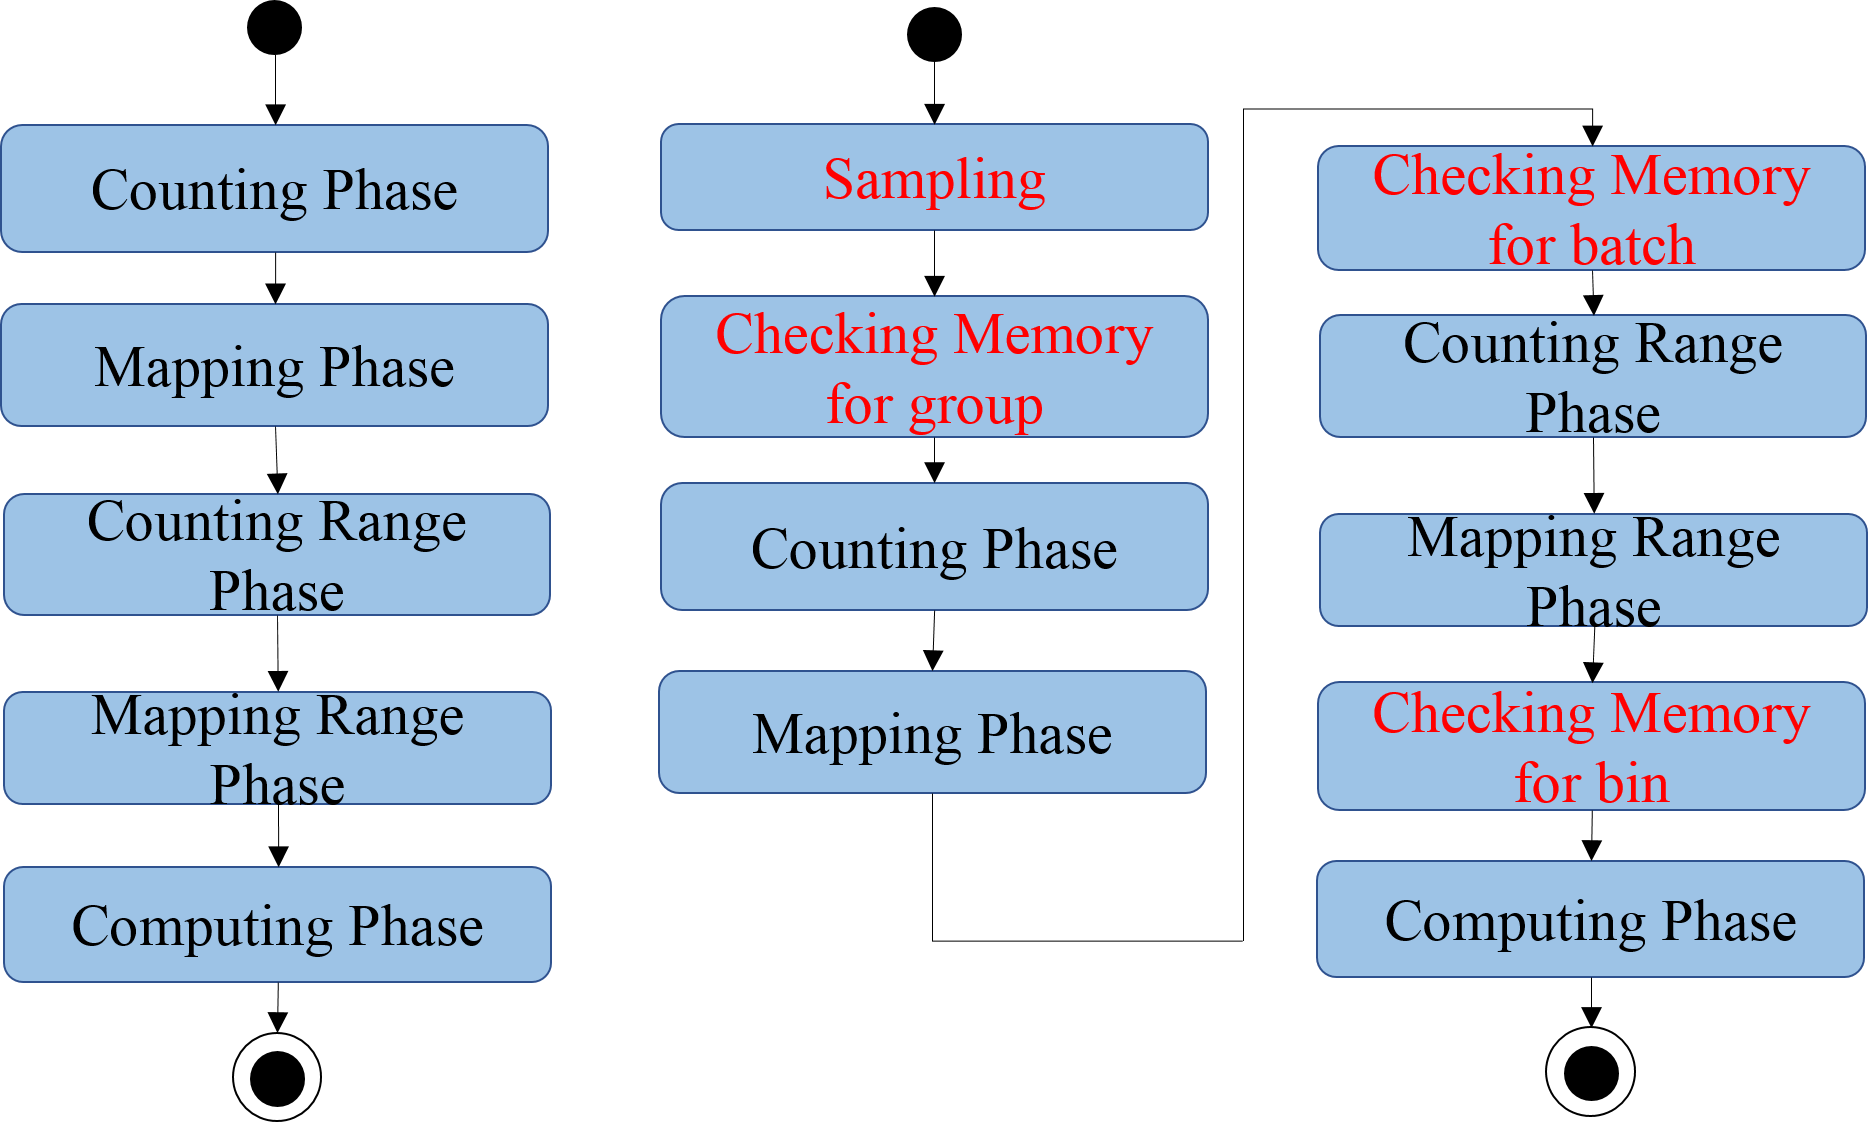
\includegraphics[scale=0.4]{image/fig_3_5}
    \caption{(a) The flow chart of multi-slab and multi-sweep-line without checking memory (b) The flow chart of multi-slab and multi-sweep-line with checking memory}
    \label{fig:fig_3_5}
\end{figure}

\subsubsection{Counting phase}
Same as the counting phase in baseline version.

\subsubsection{Mapping phase}
Same as the mapping phase in baseline version.

\subsubsection{Counting range phase}
The main task of counting range phase is counting the number of rectangles for each slab per window. We unique the \textit{x\_range array} and sort it to compute how many slabs per window before perform the main task. And then counting the number of rectangles. Like the counting phase in baseline version, each thread handles one rectangle in this window and computes the ranges it occupies. For an occupied range of index $i$, the thread increases the $i$th element in the \textit{range counter array} using atomic instruction to avoid race condition.

\subsubsection{Mapping range phase}
Unlike the counting range phase, each thread handles one slab instead of one rectangle. It can keep the order of rectangles in this slab. We need to spend much time to sort the \textit{range rectangle array} if each thread handles one rectangle using atomic instruction.

\subsubsection{Computing phase}
Same as the computing phase in baseline, but every thread only checks all rectangles within a slab.

\subsection{Multi-Sweep-Line Algorithm}
In computing phase in multi-slab version, each thread handles a slab and scan all rectangles within this slab. It is faster than computing phase in baseline version. However, it suffers from the discontinuous memory access: (1) we need to read rectangle's information and rectangles' information only sorted according to their y coordinate; (2) each thread in same warp (32 threads) access rectangle's index in \textit{range rectangle array} is not continuous because each thread handles different slabs. First condition cannot be fixed unless we save rectangles' value to range rectangle array instead of rectangles' index. This way will use amount of memory and memory is rare resource. In this optimization technique, we solve the problem in the second condition.

We modify the implementation in computing phase. Original sweep line algorithm scan rectangles one by one. We now scan 32 (size of warp in CUDA) rectangles in one time. We let each warp handle a slab and each thread in the same warp handles a rectangle, compare the value of the status variable (the value of statue is window's smaller y coordinate in the beginning), and check the rectangles (these rectangles' ymax) which are handled by the threads that their thread ID is smaller than its. After checking rectangles, each thread computes the area and adds the result to local variable. The final thread in this warp has maximum y coordinate value and update the status. After that, warp handles next 32 rectangles in this slab. Fig. \ref{fig:fig_4_2} shows the example.
\begin{figure}[h]
    \centering
    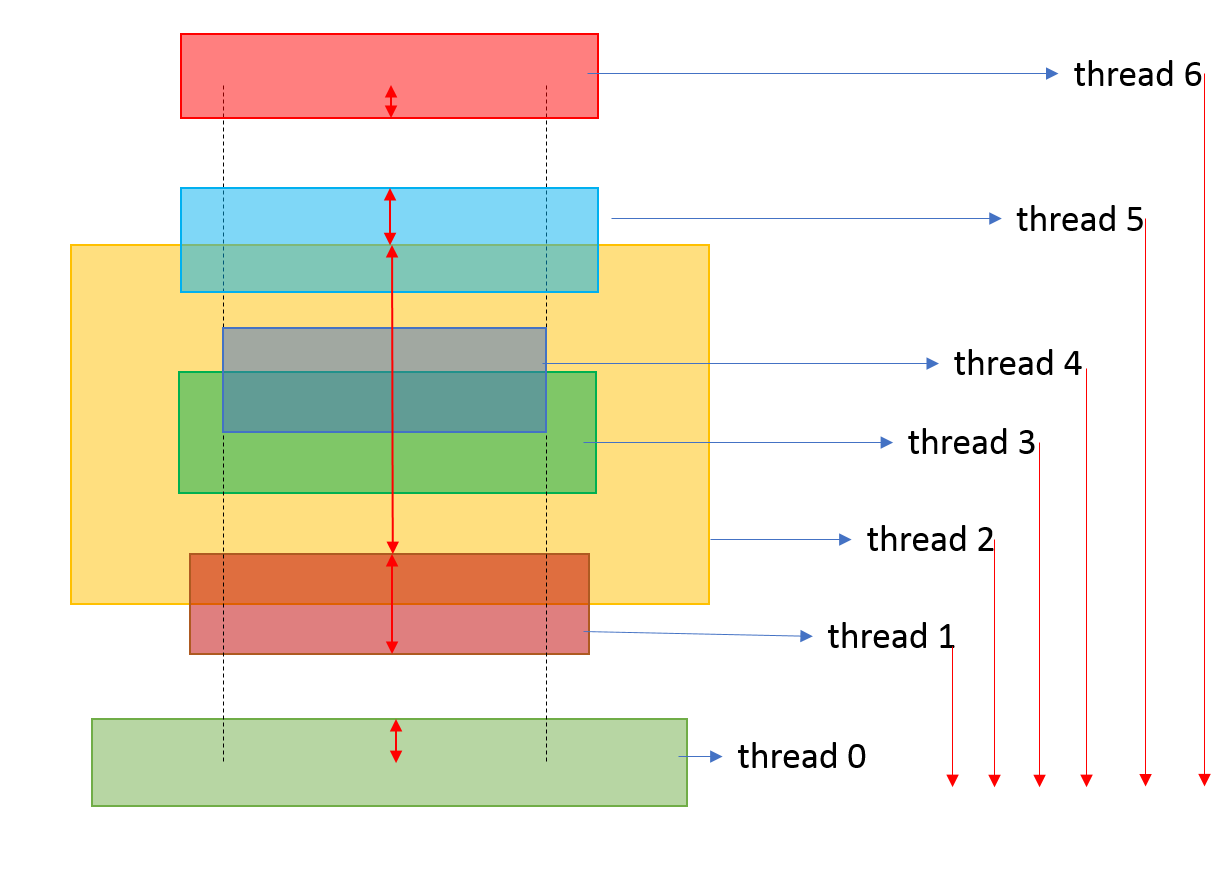
\includegraphics[scale=0.4]{image/fig_4_2.png}
    \caption{Example of computing phase using multi-sweep-line, each thread in same warp handles a rectangle in same slab (each red arrow are calculated by certain thread)}
    \label{fig:fig_4_2}
\end{figure}

% adaptive memory partition
\subsection{Checking and adaptive task partition}
The computing phase time in multi-slab and multi-sweep-line version is faster than baseline version, but it uses a lot of GPU memory to save additional arrays (i.e. the \textit{range counter array}, the \textit{range offset array}, and \textit{range rectangle array}). For example, certain test cases will generate a \textit{range rectangle array} about 60 GB. There is no such a GPU has enough global memory to store the array in one time. To solve this problem, we designed an adaptive partition method. (see Fig. \ref{fig:fig_3_5}b) The unit of our partition method is window, Fig. \ref{fig:fig_3_8} shows the schematic diagram. The pseudo code is shown in Algorithm \ref{alg:a5}.

\begin{figure}[h]
    \centering
    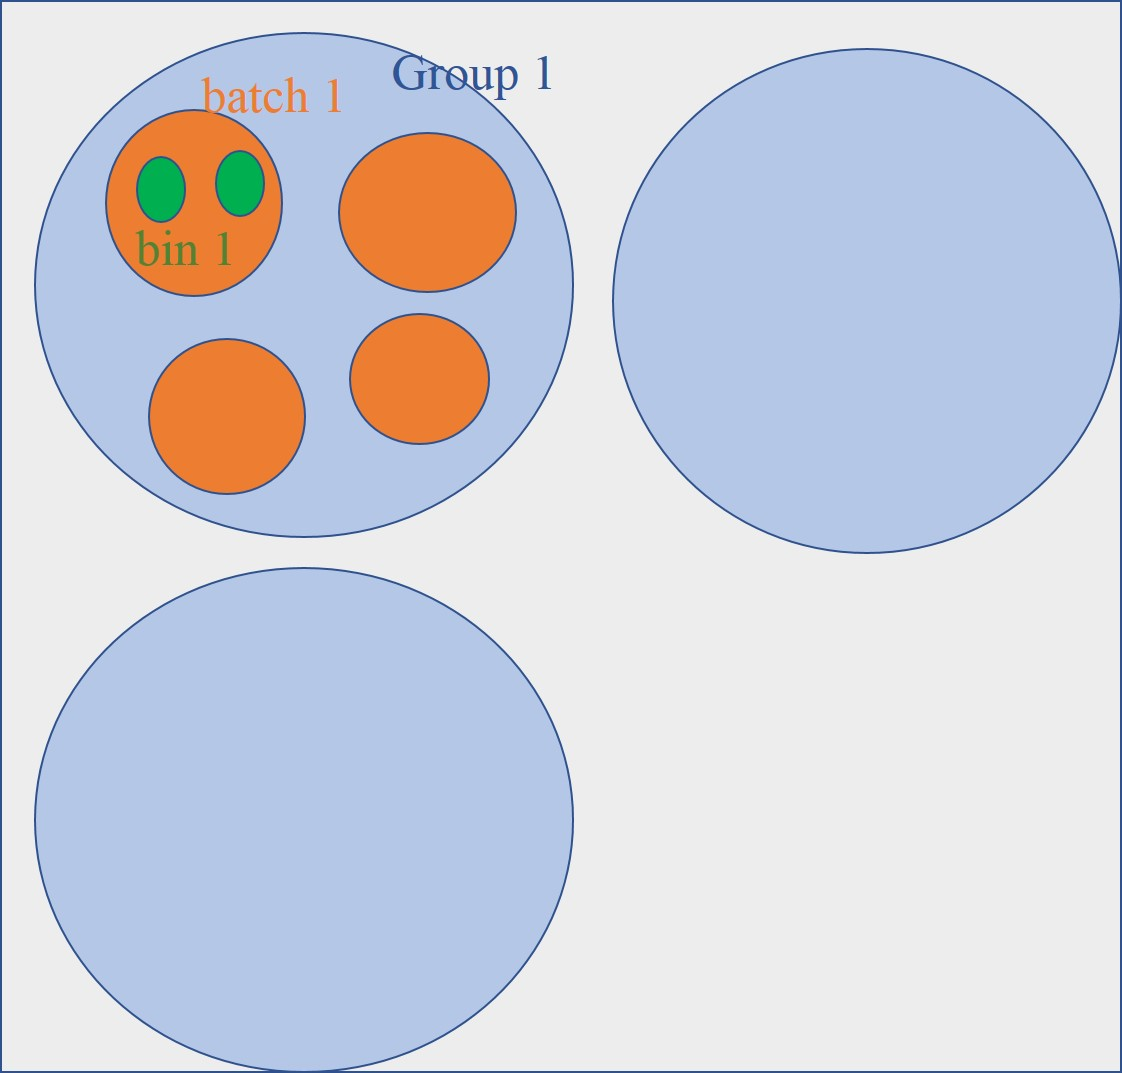
\includegraphics[scale=0.4]{image/fig_3_8.jpg}
    \caption{The schematic diagram of partition method (group, batch, and bin), which the unit is window}
    \label{fig:fig_3_8}
\end{figure}

\begin{algorithm}[H]
\label{alg:a5}
\caption{Multi-slab and multi-sweep-line with checking memory}
\DontPrintSemicolon
\renewcommand\baselinestretch{0.7}\selectfont
 \KwData{$R$: a list of rectangles for each windows}
 \KwResult{Each window's area of rectangle union}
 \SetKwFunction{FMain}{main}
 \SetKwProg{Pn}{Function}{:}{\KwRet}
 \Pn{\FMain}{
     sampling\;
     \#groups = Checking memory for windows\;
     \ForEach{group of windows}{
         sort the x value of rectangles for each window\;
         sort each window's rectangles based on y\;
         \#batch = Checking memory for slabs\;
         \ForEach{batch of windows}{
             create range\_counter array for each slab\; 
             create range\_offset array for each slab\;
             \#bin = Checking memory rectangles\;
             \ForEach{bin of windows}{
                 create range\_rectangle array for each slab\;
                 \bf{parallel} \ForEach{$W_j \in W$}{
                     $area = 0$\;
                     \bf{parallel} \ForEach{$slab (x[i-1], x[i])$}{
                         compute\_area($x[i-1], x[i]$)\;
                     }
                 }
             }
         }
     }
 }
\end{algorithm}

\subsubsection{Sampling}
\begin{table}[h!]
\centering
\begin{tabular}{|c | l |} 
 \hline
 Symbol & Meaning \\ [0.5ex] 
 \hline
 $\alpha$ & average number of rectangles per window  \\
 $\beta$ & average number of rectangles per slab in the window  \\
 $\gamma$ & average number of windows that a rectangle occupies  \\
 $N$ & number of total rectangles \\
 $M$ & number of total windows  \\ \hline
 $l^i_c$ & length of cell in the $i$th dimension  \\
 $l^i_r$ & length of rectangle in the $i$th dimension  \\ \hline
 $win\_size$ & length of each window  \\
 $win\_stride$ & interval between two adjacent windows  \\
 \hline
\end{tabular}
\caption{List of Symbols}
\label{table:symbol}
\end{table}
The memory usage in whole process we estimate is approximate $(6M + 11\alpha M + (2\alpha - 1) M\beta)$ 32 bits ($(2\alpha - 1)$ means average of maximum number of slabs in each window), where $M$ is the number of windows, $\alpha$ is the average number of rectangle per window, and $\beta$ is the average number of rectangles per slab in the window.

Given the window's size, window's stride, and the size of $l^1_c \times l^2_c$, where $l^i_c$ is the length of cell in the $i$th dimension and symbol stands for the multiplication sign between scalars, $M$ can be calculated as
\begin{equation}
M = \left(\left\lceil{\frac{l^1_c - win\_size}{win\_stride}}\right\rceil + 1\right) \times \left(\left\lceil{\frac{l^2_c - win\_size}{win\_stride}}\right\rceil + 1\right).
\end{equation}
Similarly, given the size of a rectangle r $l^1_r \times l^2_r$, where $l^i_r$ is the length of r in the $i$th dimension and symbol stands for the multiplication sign between scalars, the number of windows occupied by r can be estimated using
\begin{equation}
\left(\left\lceil{\frac{l^1_r - win\_size}{win\_stride}}\right\rceil + 1\right) \times \left(\left\lceil{\frac{l^2_r - win\_size}{win\_stride}}\right\rceil + 1\right) \mbox{, if $l^i_c > win\_size$}.
\end{equation}
Thus, $\gamma$ is defined as 
\begin{equation}
\gamma = \frac{1}{N}\sum_{r \in R} \left(\left(\left\lceil{\frac{l^1_r - win\_size}{win\_stride}}\right\rceil + 1\right) \times \left(\left\lceil{\frac{l^2_r - win\_size}{win\_stride}}\right\rceil + 1\right)\right),
\end{equation}
where $R$ denotes the set of $N$ rectangles in the cell. Then, $\alpha$ can be computed as 
\begin{equation}
\alpha = \frac{N * \gamma}{M}
\end{equation}
To reduce the calculational cost and increase accuracy, we take a simple random sample of size 1024 from $M$ windows to estimate $\alpha$ and offload sampling phase onto the GPU.

Based on the same consideration, we using $\alpha$ to estimate $\beta$ instead of calculating $\beta$ using sample method. We assume average number of slabs is $(2\alpha - 1)$ per window (because each window evenly has $\alpha$ rectangles). The value of $\beta$ is between $\frac{\alpha}{2\alpha-1} \sim \frac{\alpha^2}{2\alpha-1}$, which means best case and worst case(like Fig. \ref{fig:fig_3_6}). And we take the middle of these two number to denote $\beta$.
\begin{figure}[h]
    \centering
    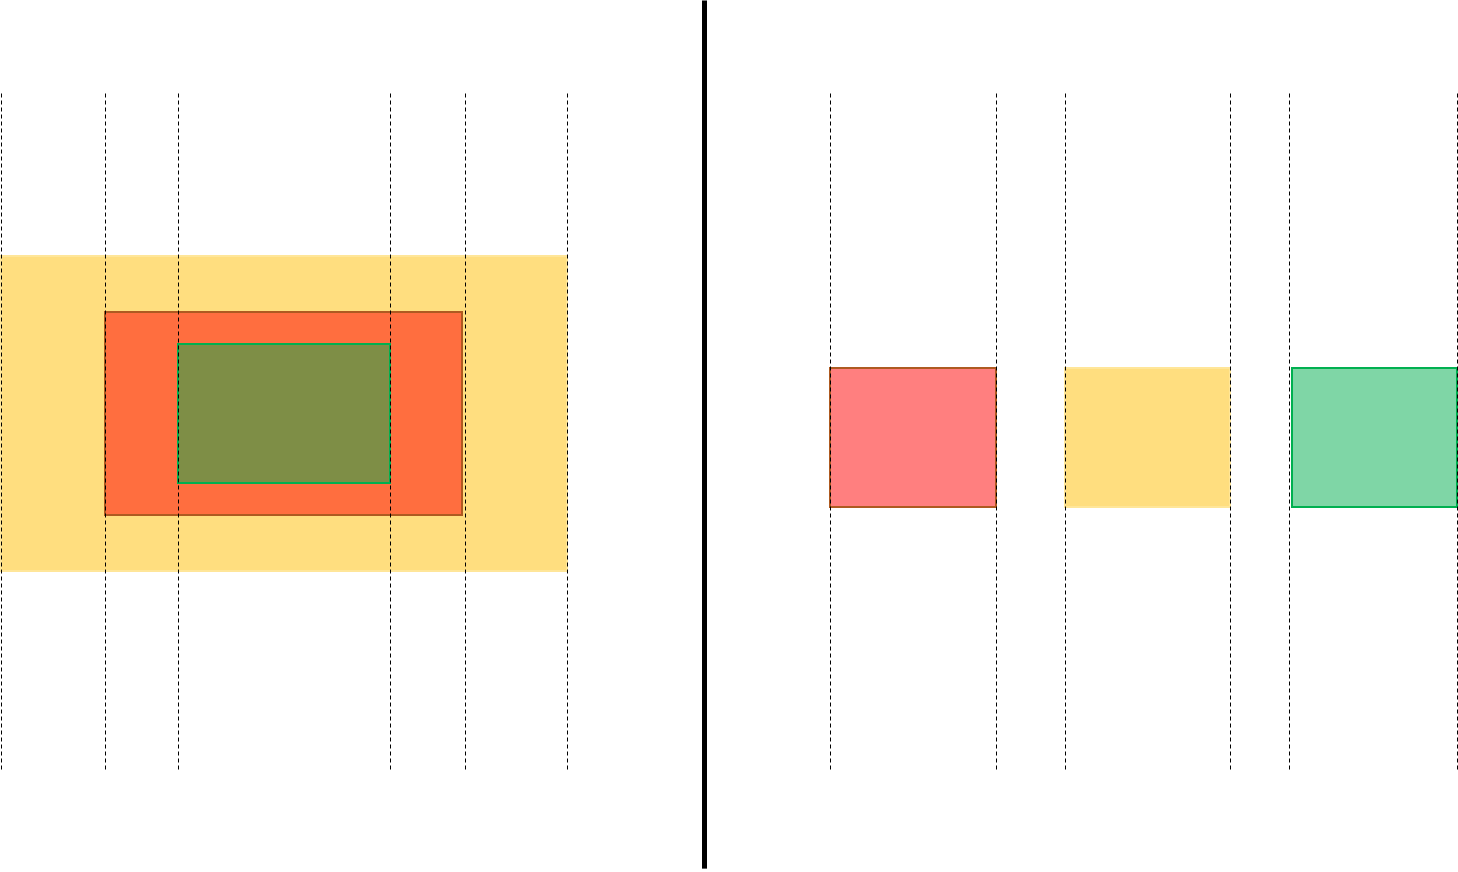
\includegraphics[scale=0.4]{image/fig_3_6}
    \caption{One of the worst case (left) and best case (right) of overlapping}
    \label{fig:fig_3_6}
\end{figure}

\subsubsection{Checking memory for windows (group)}
Using $\alpha$ can estimate total memory usage except \textit{range rectangle array}, \textit{range offset array} and \textit{range counter array} (because these arrays almost larger than GPU memory, and we check these three arrays in checking memory for slabs and rectangles). If memory is not enough, we partition windows equally.

\subsubsection{Checking memory for slabs (batch)}
If memory is not enough for \textit{range counter array} and \textit{range offset array}, this phase will use $\beta$ to determinate how many parts does the workload be divided and adaptive partition task. We use $\beta$ to make a decision because we do not want the process partition task in checking memory 3 phase after divide the work in this phase.

\subsubsection{Checking memory for rectangles (bin)}
If \textit{range rectangle array} is larger than free memory, this phase will adaptive partition task according to \textit{range offset array}.

It should be noted that we do not remove any array, which is complete computed before checking memory for slabs or for rectangles, because all the information can be reuse and we do not want to repeat the calculation.

%%%%%%%%%%%%%%%%%%%%%%%%%%%%%%%%%%%%%%%%%
\section{Performance Optimization}
In this section, we present three optimization techniques to further enhance the GPU performance. The first technique uses fast segmented sort to speed up the sorting time. The second technique reduces the usage of atomic instruction which can break performance. The third technique modifies the implementation of computing phase in multi-sweep-line version to improve the performance.
% segment sort
\subsection{Fast segmented sort}
Hou et. al. \cite{Hou2017FastSS} presented an adaptive segmented sort mechanism for GPUs, whose key techniques contain: (1) a differentiated method for different segment lengths to eliminate load imbalance, thread divergence, and irregular memory access; and (2) an algorithm that extends sorting networks to support N-to-M data-thread binding and thread communication at GPU register level. Fig. \ref{fig:fig_4_1} shows the overview of their design. We modify their source code and integrate our algorithm with it to speed up the sorting time.
\begin{figure}[h]
    \centering
    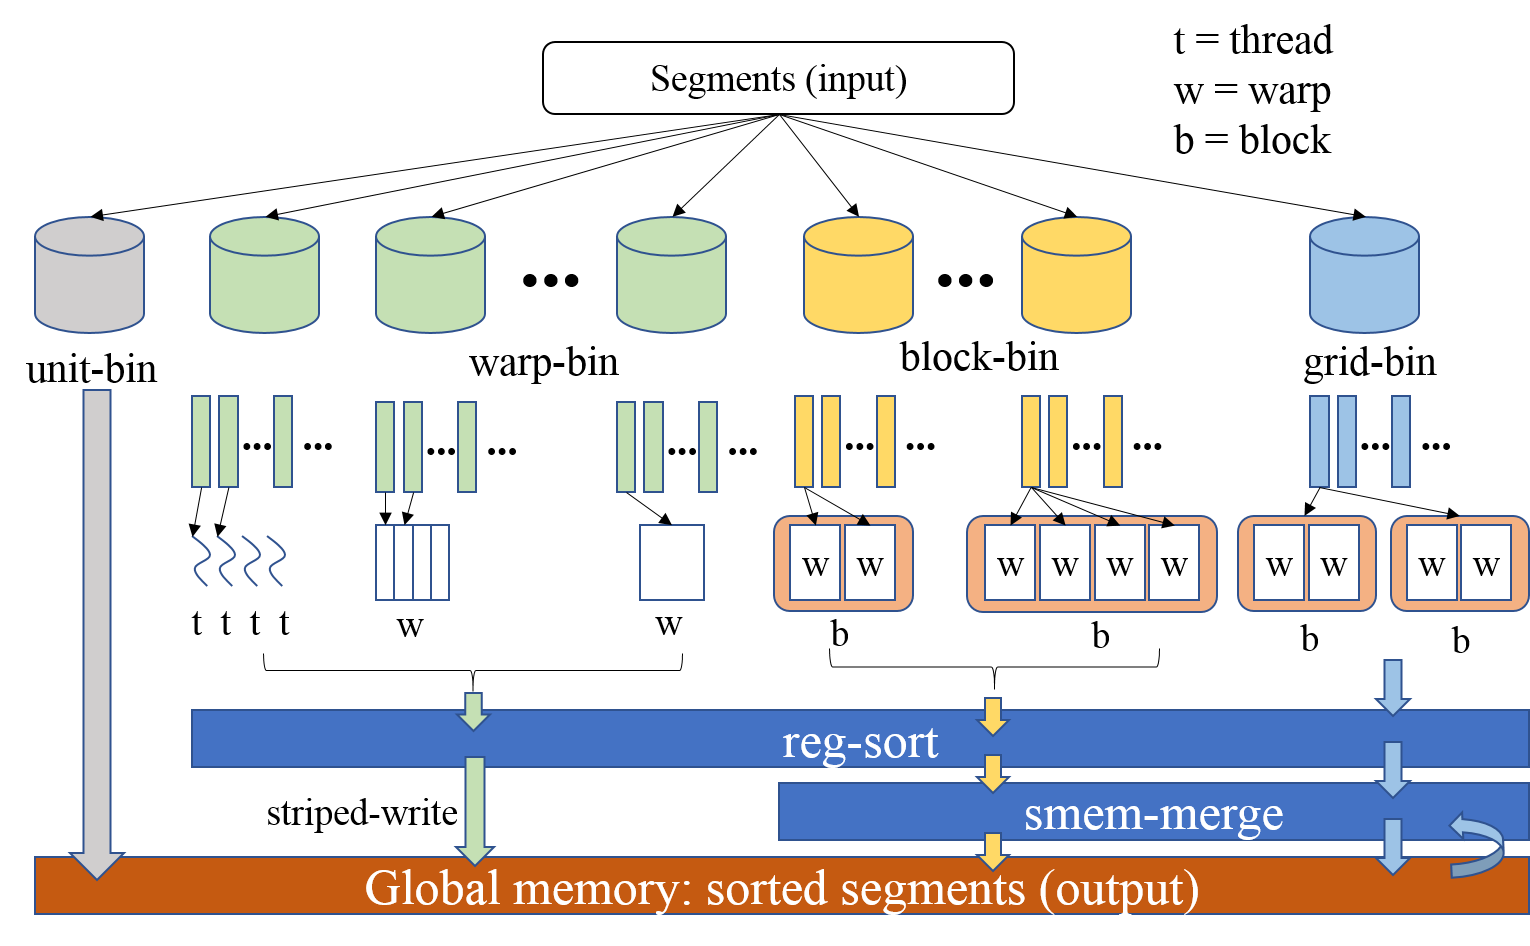
\includegraphics[scale=0.4]{image/fig_4_1.png}
    \caption{Overview of fast segmented sort}
    \label{fig:fig_4_1}
\end{figure}

% avoid atomic
\subsection{Reducing atomic instruction}
In counting range phase, change the implementation similar as the mapping range phase in multi-slab version, now each thread handles one slab instead of one rectangle. This way can avoid to use atomic instruction, which breaks performance when using frequently, to speed up the computing time.

% load balance
\subsection{Load balance}
The task of checking the rectangles is imbalance. The 32rd thread needs to run 31 times and first thread no needs to do anything. We use shuffle instruction to make it load balance, and it can avoid to synchronize threads or access violate shared memory which the latency is higher than register operation. Fig. \ref{fig:fig_4_3} shows the steps of using shuffle to make the task be load balance.
\begin{figure}[h]
    \centering
    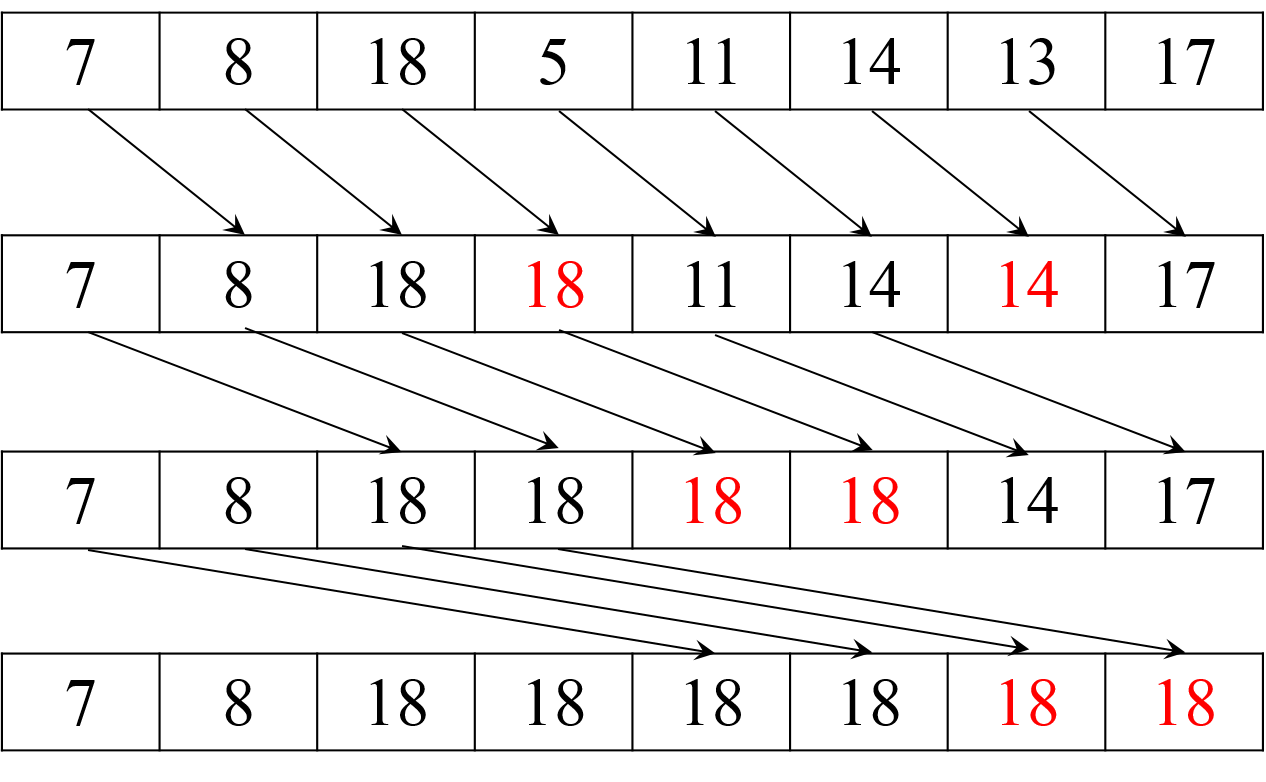
\includegraphics[scale=0.4]{image/fig_4_3.png}
    \caption{Example of load balance in parallel prefix max using shfl\_up instruction }
    \label{fig:fig_4_3}
\end{figure}

%%%%%%%%%%%%%%%%%%%%%%%%%%%%%%%%%%%%%%%%%%%%%%%%55
\section{Calculating right triangle union area in CPU}
In our GPU implementations, we only deal with rectangles and do not consider right triangles. In order to fully use computing resource, we calculate right triangles using CPU. First, we decompose vertical trapezoids into one rectangle and two right triangles, and deal with them as three rectangles on GPU because we want to use \textit{rectangle array} to map window faster and reduce computing time. We add a flag to identify the object which is rectangle or one of the four types of right triangles. Then, each triangle is computed union area as rectangle on GPU, so we need to subtract the difference area of the triangle. For this purpose, we scan all triangle in each window, and use line sweep algorithm to obtain the difference area which is not covered by other objects in this window.

\subsection{Finding out intersection points}
It is not necessary to find out the intersection points with all objects in this window, we only need to consider the object which is intersection with the triangle's boundary (to simplify the calculation, we use rectangle's boundary to represent the triangle). We classify edges into two categories, horizontal and hypotenuse, to reduce the computing task.  If the line is belong to horizontal, it only need to find intersection points with lines which are belong to hypotenuse. We sort the intersection points and x axis value of each object after we find out all intersection points.

\subsection{Calculating area}
In this step, we need to calculate this triangle's area which is not covered by other rectangles and triangles. We compute the total area in each slab at first, and using line sweep algorithm to calculate the union area and subtract it to the total area. We also check the window's boundary. Finally, we can obtain the value which is needed to subtract the result from GPU.

In order to deal with the union area between triangles, we make the triangle as rectangle after we already calculate its area. (see Fig. \ref{fig:fig_3_7})

\begin{figure}[h]
    \centering
    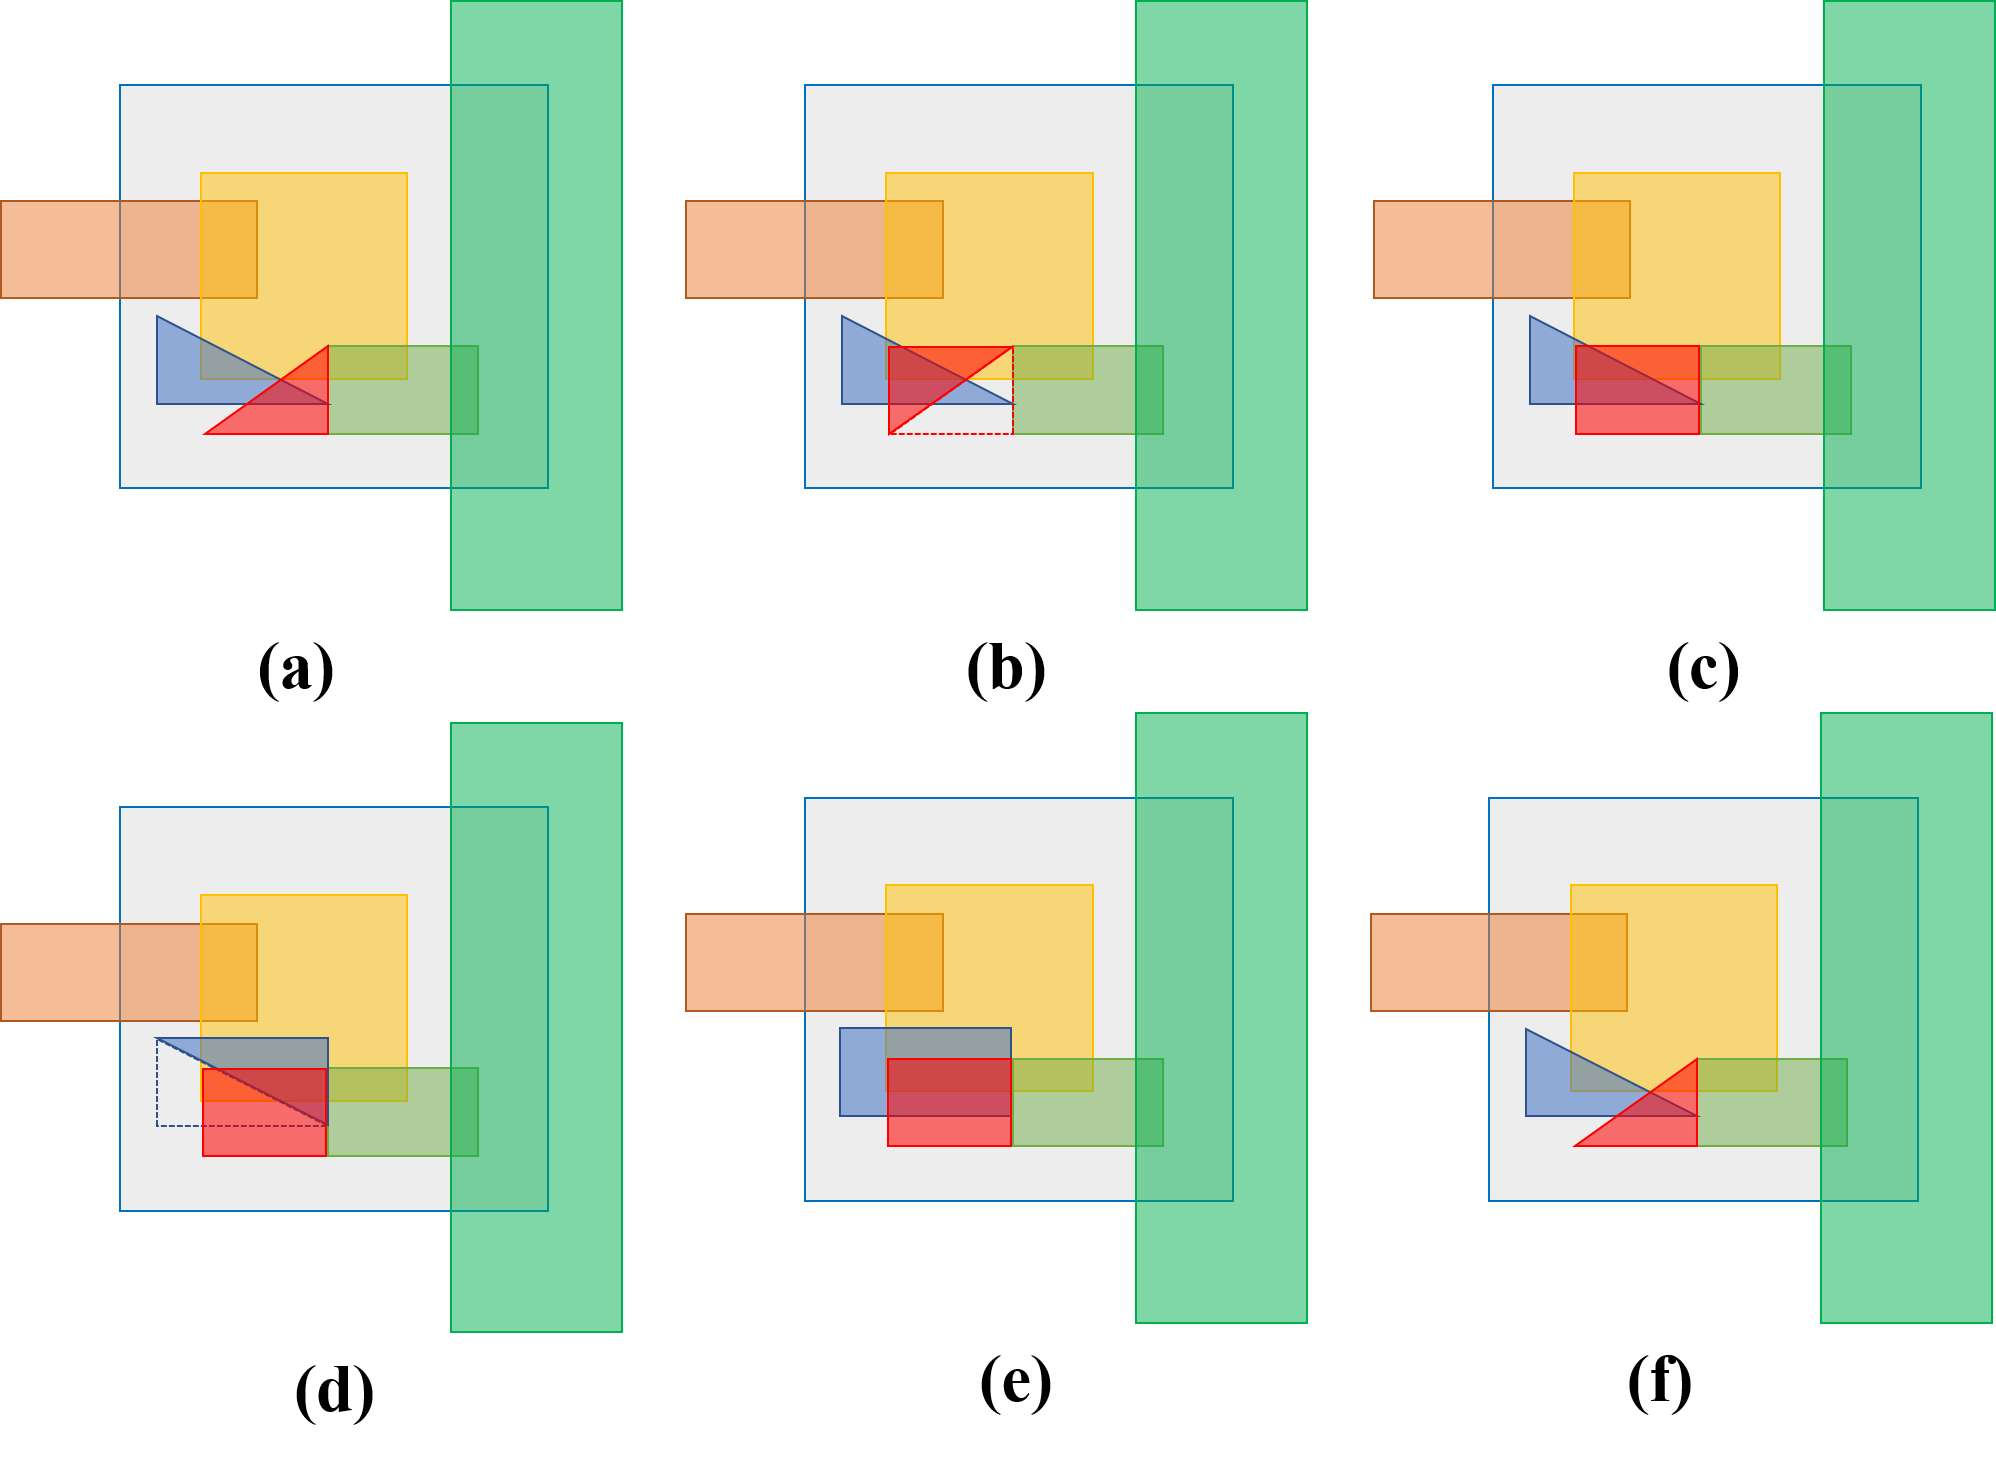
\includegraphics[scale=0.4]{image/fig_3_7}
    \caption{(a) origin input data in the window
(b) calculating the difference area of red triangle 
(c) treat red triangle as rectangle after computing its difference area
(d) calculating the difference area of blue triangle
(e) treat blue triangle as rectangle after computing its difference area 
(f) the input data does not change
}
    \label{fig:fig_3_7}
\end{figure}